\section{Parallellization}
The most time consuming part of my program is in the function called findForces(). Here there is two four loops (one triple- and one quadruple- for loop), that
runs through all the particles and calculates the forces. In parallellizing the code we seem to have to options; we can divide the system into cells (larger than the cells we already have), and calculate the forces 
in these cells in parallel (with the aid of MPI to communicate), or we can let the program run in serial except when we calculate the forces. I have chosen the latter option, where I use openMP to parallellize the loops.
This is a much easier solution, because it just means adding a few lines of code in my original code. The back side to this solution is that it requires that we work on a shared memory computer, while the solution with
MPI will run on a cluster. For now I am working on a shared memory computer, so it is fine, but if I want to run for a larger system I will consider using MPI.\\
\subsection{Efficiency}
If it takes an amount of time, $T(N,P)$, to find the new state in a molecular dynamics code, the speed of the simulation may be characterized by
\begin{align}
 S_P = T(N,1)/T(N,P)\nonumber
\end{align}


where N is the number of atoms and P is the number of parallel processes.\\
The parallel efficiency of the method is
\begin{align}
 E_P = S_P/P.
\end{align}

\begin{figure}[H]
 \subfigure[Time spent with four parallel processes.]{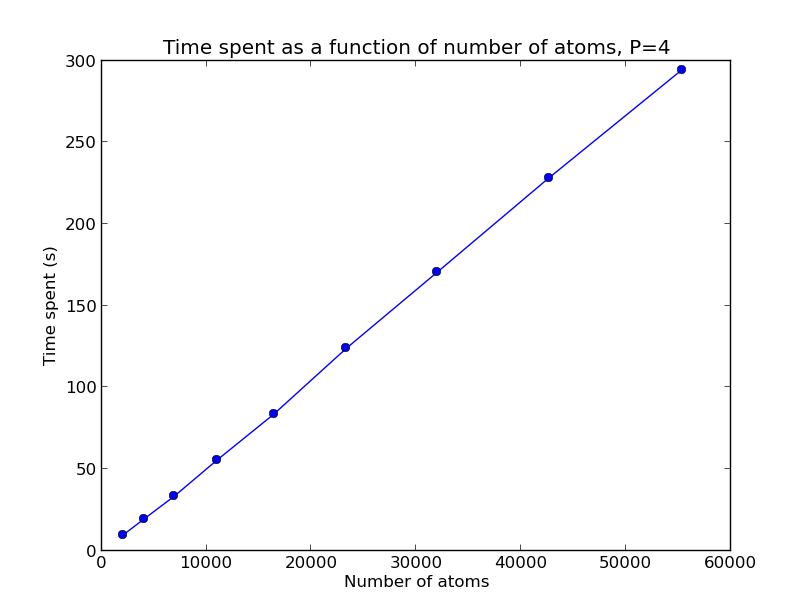
\includegraphics[width=0.3\textwidth]{figures/time_spent_P_4.png}}
  \subfigure[The speed with four parallel processes ]{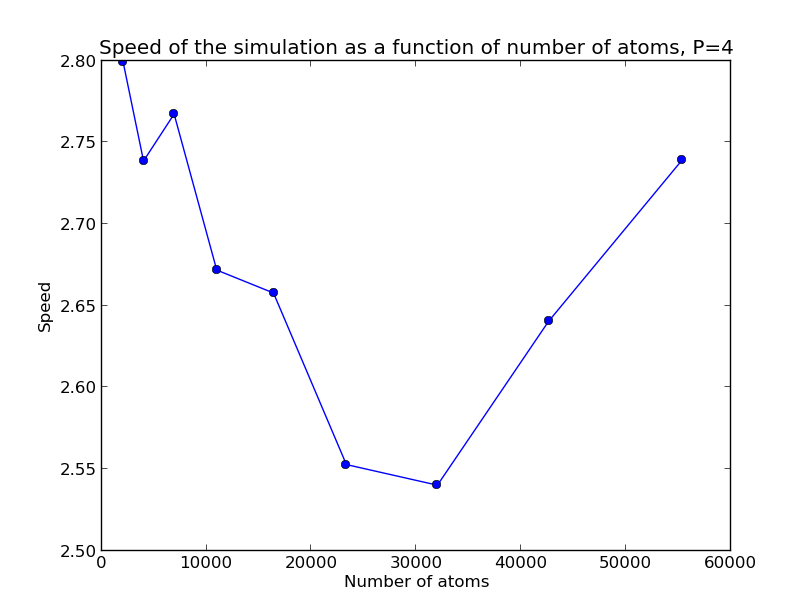
\includegraphics[width=0.3\textwidth]{figures/speed_P_4.png}}
  \subfigure[The efficiency with four parallel processes]{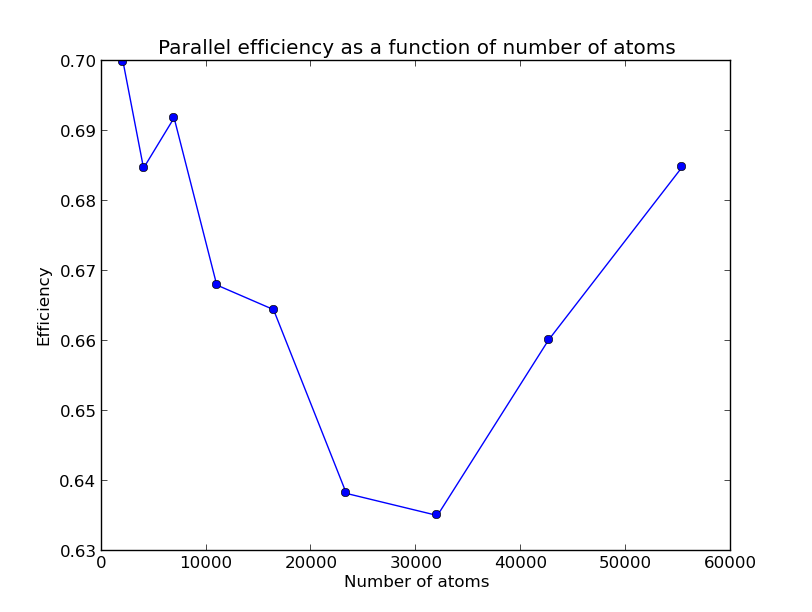
\includegraphics[width=0.3\textwidth]{figures/eff_P_4.png}}
  
     \subfigure[Time spent with $N=4\cdot10^3$, varying P.]{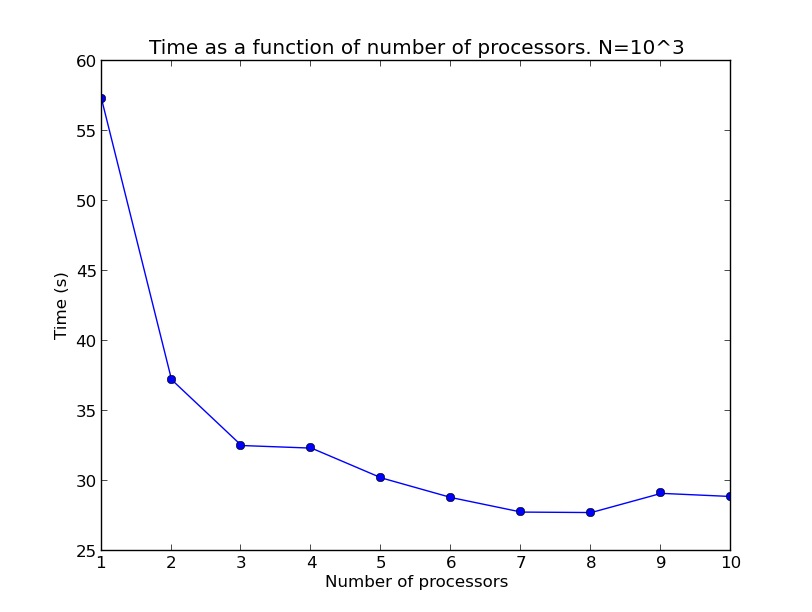
\includegraphics[width=0.3\textwidth]{figures/time_spent_N_1000.png}}
  \subfigure[Speed with $N=4\cdot10^3$, vaying P.]{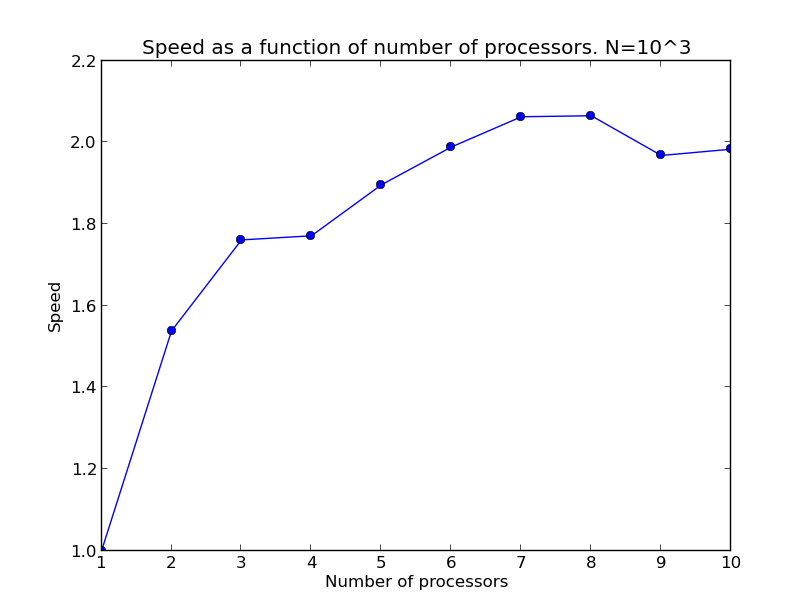
\includegraphics[width=0.3\textwidth]{figures/speed_N_1000.png}}
  \subfigure[Efficiency with $N=4\cdot10^3$, varying P.]{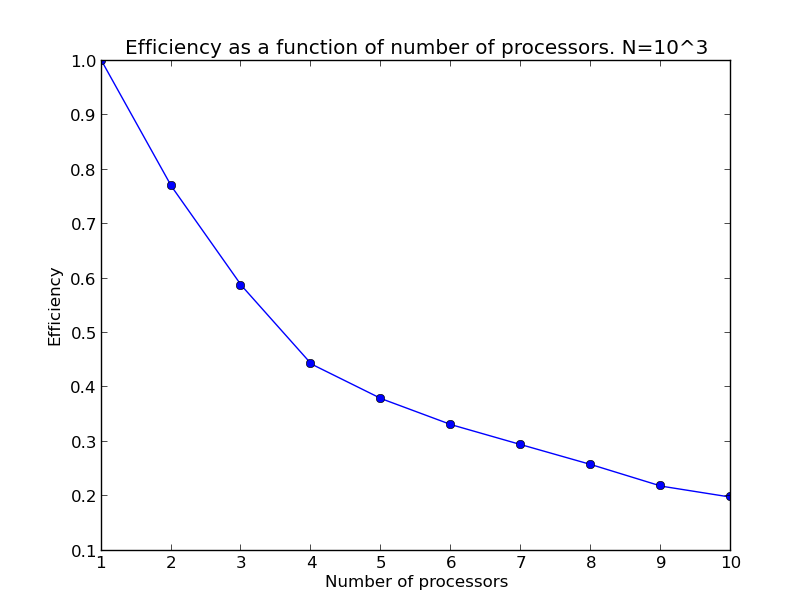
\includegraphics[width=0.3\textwidth]{figures/eff_N_1000.png}}
  
   \subfigure[Time spent for P=128N, varying both N and P.]{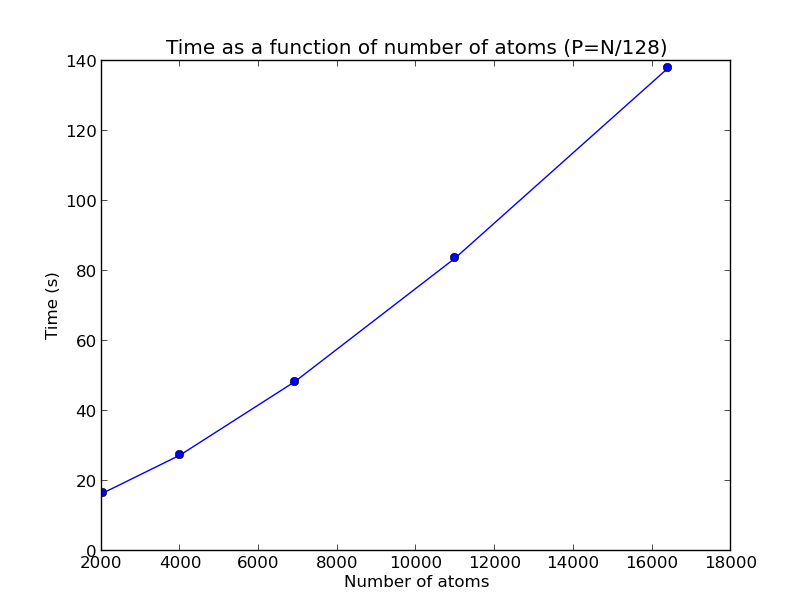
\includegraphics[width=0.3\textwidth]{figures/time_PratioN_128.png}}
  \subfigure[Speed for P=128N, varying both N and P.]{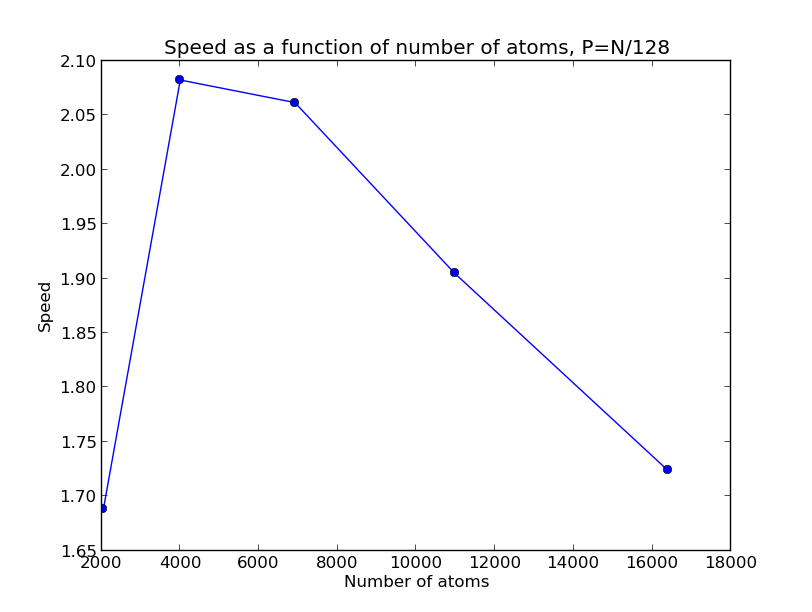
\includegraphics[width=0.3\textwidth]{figures/speed_PratioN_128.png}}
  \subfigure[Efficiency for P=128N, varying both N and P.]{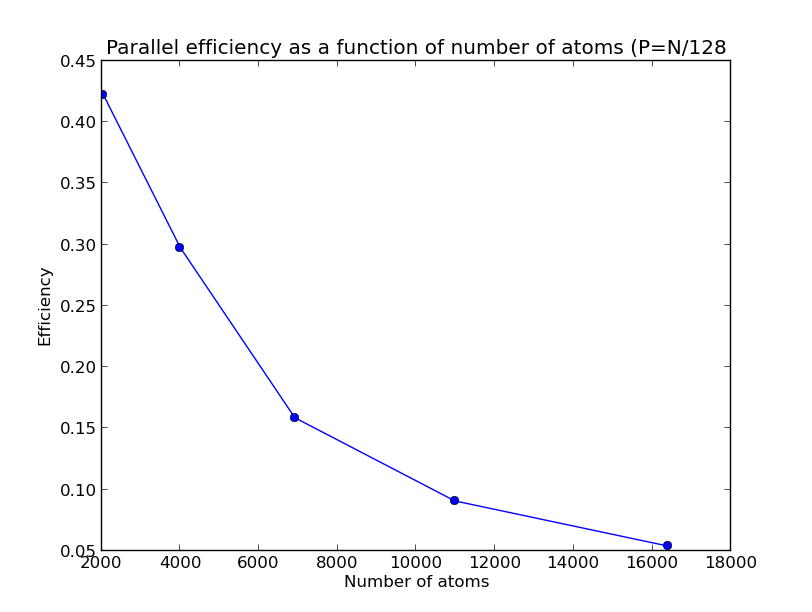
\includegraphics[width=0.3\textwidth]{figures/eff_PratioN_128.png}}
  

 \caption{Testing the parallellized program by varying P and N. }
 \label{g_pict}
\end{figure}






